\documentclass{article}
\usepackage{xcolor}
\usepackage{listings}
\usepackage{geometry}
\usepackage{graphicx}

\lstdefinestyle{BashInputStyle}{
  language=bash,
  basicstyle=\small\sffamily,
  frame=tb,
  columns=fullflexible,
  backgroundcolor=\color{gray!20},
  linewidth=0.9\linewidth,
}

\author{ Group 22 }
\date{}
\title{Basic Computing Tools}
\begin{document}
	
	\maketitle
	
	\section{Bash}
        \subsection{Introduction}
Bash is a Unix shell and command language written by Brian Fox for the GNU Project as a free software replacement for the Bourne shell. Released in 1989, it has been distributed widely as the shell for the GNU operating system and as a default shell on Linux and OS X. It was announced during the 2016 Build Conference that Windows 10 has added a Linux subsystem which fully supports Bash and other Ubuntu binaries running natively in Windows. In the past, and currently, it has also ported to Microsoft Windows and distributed with Cygwin and MinGW, to DOS by the DJGPP project, to Novell NetWare and to Android via various terminal emulation applications. In the late 1990s, Bash was a minor player among multiple commonly used shells; at present Bash has overwhelming favor.
\begin{enumerate}
    \item
        For quick display of files:
        \begin{lstlisting}[style=BashInputStyle]
            \$ cat helloworld.sh
            #!/bin/bash
            echo Hello World
        \end{lstlisting}
\end{enumerate}
    \subsection{GREP}
    grep is a command-line utility for searching plain-text data sets for lines matching a \textbf{regular expression}. Grep was originally developed for the Unix operating system, but is available today for all Unix-like systems. Its name comes from the ed command g/re/p (\textbf{g}lobally search a \textbf{re}gular expression and \textbf{p}rint), which has the same effect: doing a global search with the regular expression and printing all matching lines.

Some basic grep commands are as follows:
\begin{enumerate}
    \item
        For basic string search:
        \begin{lstlisting}[style=BashInputStyle]
            \$ grep "literal\_string" filename
        \end{lstlisting}
    \item
        For case insensitive search:
        \begin{lstlisting}[style=BashInputStyle]
            \$ grep -i "string" filename
        \end{lstlisting}
    \item
        For regular expressions:
        \begin{lstlisting}[style=BashInputStyle]
            \$ grep  "REGEX" filename
        \end{lstlisting}
    \item
        To display N lines after match:
        \begin{lstlisting}[style=BashInputStyle]
            \$ grep  -A <N> "string" filename
        \end{lstlisting}
    \item
        To display N lines before match:
        \begin{lstlisting}[style=BashInputStyle]
            \$ grep  -B <N> "string" filename
        \end{lstlisting}
    \item
        To display lines which do not contain match:
        \begin{lstlisting}[style=BashInputStyle]
            \$ grep  -v -e "pattern" -e "pattern" filename
        \end{lstlisting}
    \item
        Counting number of matches:
        \begin{lstlisting}[style=BashInputStyle]
            \$ grep  -c "pattern" filename
        \end{lstlisting}
    \item
        To display N lines before match:
        \begin{lstlisting}[style=BashInputStyle]
            \$ grep  -B <N> "string" filename
        \end{lstlisting}
\end{enumerate}
    \subsection{SED}
    sed (stream editor) is a Unix utility that parses and transforms text, using a simple, compact programming language. \textbf{sed} was developed from 1973 to 1974 by Lee E. McMahon of Bell Labs, and is available today for most operating systems. sed was based on the scripting features of the interactive editor ed ("editor", 1971) and the earlier qed ("quick editor", 1965–66). sed was one of the earliest tools to support regular expressions, and remains in use for text processing, most notably with the substitution command. Other options for doing "stream editing" include AWK and Perl.

    \begin{enumerate}
        \item
            To match files and replace:
                \begin{lstlisting}[style=BashInputStyle]
                     sed  -e   ‘s/<find expression>/<replace expression>/’ filename
                \end{lstlisting}
        \item
            To use the match as a part of replace string, we can use the following command:
                \begin{lstlisting}[style=BashInputStyle]
                    sed -n -e  's/United States/& of America/p' country.txt
                    United States of America
                \end{lstlisting}
          \item
            To convert lower case letters to upper case:
                \begin{lstlisting}[style=BashInputStyle]
                    sed 'y/ul/UL/' file.txt
                \end{lstlisting}
  \end{enumerate}
  \subsection{AWK}
AWK is an interpreted programming language designed for text processing and typically used as a data extraction and reporting tool. It is a standard feature of most Unix-like operating systems.

The AWK language is a data-driven scripting language consisting of a set of actions to be taken against streams of textual data – either run directly on files or used as part of a pipeline – for purposes of extracting or transforming text, such as producing formatted reports. The language extensively uses the string datatype, associative arrays (that is, arrays indexed by key strings), and regular expressions. While AWK has a limited intended application domain and was especially designed to support one-liner programs, the language is Turing-complete, and even the early Bell Labs users of AWK often wrote well-structured large AWK programs.
\begin{figure*}[!h]
	\begin{center}
		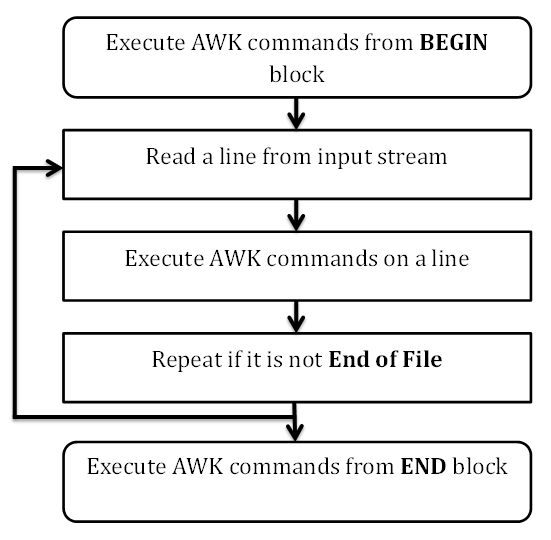
\includegraphics[width=0.4\columnwidth]{awk_workflow}
	\end{center}
	\caption{Awk Workflow}
        \label{fig:shapes}
\end{figure*}
    \begin{enumerate}
        \item
            Printing columns:
                \begin{lstlisting}[style=BashInputStyle]
                     awk '/a/ {print $3 "\t" $4}' marks.txt 
                \end{lstlisting}
        \item
            Adding variables:
                \begin{lstlisting}[style=BashInputStyle]
                     awk '/a/{++cnt} END {print "Count=", cnt}' marks.txt
                \end{lstlisting}
  \end{enumerate}

    \section{Octave}
	\section{Latex}
	\LaTeX is a typesetting system that is very suitable for producing scientific and mathematical documents of high typographical quality. It is also suitable for producing all sorts of other documents, from simple letters to complete books.\\
	\\
	\LaTeX enables authors to typeset and print their work at the highest typographical quality, using a predefined, professional layout. \LaTeX was originally written by Leslie Lamport.\\
	
	\LaTeX commands are case sensitive, and take one of the following two formats:
	\begin{enumerate}
		\item They start with a backslash \textbackslash and then have a name consisting of
		letters only. Command names are terminated by a space, a number or
		any other 'non-letter.'
		\item They consist of a backslash and exactly one non-letter.
		\item Many commands exist in a 'starred variant' where a star is appended
		to the command name.
	\end{enumerate}
	
		\section{gnuplot}
		\section{XFig}
		\section{HTML}
		\section{Git}
		\section{BitBucket}
		
	\end{document}
